%2multibyte Version: 5.50.0.2960 CodePage: 1252
%Bibliography and citation formating
% Custom date format for date field
% Defining month year date format
%\usepackage{tikz}                                        % Timelines and other drawings
%\usetikzlibrary{decorations}                             % Formating for Tikz

\documentclass[11pt]{book}%
\usepackage[%dvipdfm,  %pdflatex,pdftex这里决定运行文件的方式不同
%pdfstartview=FitH,
%CJKbookmarks=true,\eqref{}
%bookmarksnumbered=true,
%bookmarksopen=true,
colorlinks, %注释掉此项则交叉引用为彩色边框(将colorlinks和pdfborder同时注释掉)
pdfborder=001,   %注释掉此项则交叉引用为彩色边框
linkcolor=blue,
anchorcolor=blue,
citecolor=blue
]{hyperref}  
\usepackage{cite} 
\usepackage{hyperref}
\usepackage{float,booktabs} 
\usepackage{amsfonts}
\usepackage{amsmath}
\usepackage{amssymb}
\usepackage{geometry}
\usepackage{graphicx}
\usepackage{booktabs}
\usepackage{lscape}
\usepackage{longtable}
\usepackage{multirow}
\usepackage{appendix}
\usepackage{threeparttable}
\usepackage{caption}
\usepackage{sidecap}
\usepackage{accents}
\setcounter{MaxMatrixCols}{30}
%TCIDATA{OutputFilter=latex2.dll}
%TCIDATA{Version=5.50.0.2960}
%TCIDATA{Codepage=1252}
%TCIDATA{CSTFile=LaTeX article (bright).cst}
%TCIDATA{Created=Thursday, March 01, 2007 10:16:25}
%TCIDATA{LastRevised=Monday, May 16, 2016 17:39:06}
%TCIDATA{<META NAME="GraphicsSave" CONTENT="32">}
%TCIDATA{<META NAME="SaveForMode" CONTENT="1">}
%TCIDATA{BibliographyScheme=Manual}
%TCIDATA{<META NAME="DocumentShell" CONTENT="Standard LaTeX\Standard LaTeX Article">}
%TCIDATA{Language=American English}
%BeginMSIPreambleData
\providecommand{\U}[1]{\protect\rule{.1in}{.1in}}
%EndMSIPreambleData
\newcommand{\ra}[1]{\renewcommand{\arraystretch}{#1}}
\newtheorem{theorem}{Theorem}
\newtheorem{acknowledgement}[theorem]{Acknowledgement}
\newtheorem{algorithm}[theorem]{Algorithm}
\newtheorem{assumption}{Assumption}
\newtheorem{axiom}[theorem]{Axiom}
\newtheorem{case}[theorem]{Case}
\newtheorem{claim}[theorem]{Claim}
\newtheorem{conclusion}[theorem]{Conclusion}
\newtheorem{condition}[theorem]{Condition}
\newtheorem{conjecture}[theorem]{Conjecture}
\newtheorem{corollary}[theorem]{Corollary}
\newtheorem{criterion}[theorem]{Criterion}
\newtheorem{definition}[theorem]{Definition}
\newtheorem{example}[theorem]{Example}
\newtheorem{exercise}[theorem]{Exercise}
\newtheorem{lemma}{Lemma}
\newtheorem{notation}[theorem]{Notation}
\newtheorem{problem}[theorem]{Problem}
\newtheorem{proposition}[theorem]{Proposition}
\newtheorem{remark}{Remark}
\newtheorem{solution}[theorem]{Solution}
\newtheorem{summary}[theorem]{Summary}
\newenvironment{proof}[1][Proof]{\noindent \textbf{#1.} }{\  \rule{0.5em}{0.5em}}
\newtheorem{thm}{Theorem}
\newtheorem{ex}{Example}
\newtheorem{defi}{Definition}
\newtheorem{assu}{Assumption}
\newtheorem{lem}{Lemma}
\newtheorem{prop}{Proposition}
\newtheorem{corol}{Corollary}
\geometry{left=0.8in, right=1.0in, top=1.0in, bottom=1.0in}
\pagenumbering{arabic}
\DeclareMathOperator*{\plim}{plim}
\pagenumbering{arabic}
\usepackage{authblk}
\usepackage[T1]{fontenc}
\usepackage[utf8]{inputenc}
\begin{document}
\title{	Regression Discontinuity Designs}

\author{Zhi  CAO}
\affil{All suggestions are welcome: zhicao@link.cuhk.edu.hk}

\date{
\today
}

\maketitle

\newpage
\section*{Acknowledgement}
 This note is adapted from the following literature and lecture notes:
\begin{itemize}
	\item Imbens, G. W., \& Lemieux, T. (2008). Regression discontinuity designs: A guide to practice. Journal of econometrics, 142(2), 615-635.
	
	\item Lee, D. S., \& Lemieux, T. (2010). Regression discontinuity designs in economics. Journal of economic literature, 48(2), 281-355.
	
	\item Angrist, J. D., \& Pischke, J. S. (2008). Mostly harmless econometrics. Princeton university press.
	
	\item 
\end{itemize}

Other recommended material:
\begin{itemize}
	\item Regression Discontinuity Designs(RD Packages): https://rdpackages.github.io/
\end{itemize}



	\thispagestyle{empty}
\newpage
\tableofcontents

\newpage
\pagenumbering{arabic}

\chapter{Regression Discontinuity Designs}
\section{Setup}
\subsection{Basic}
Our discussion will frame the RD design in the context of the modern literature on causal effects and treatment effects, using the Rubin Causal Model (RCM) set up with potential outcomes(Rubin, 1974; Holland, 1986; Imbens and Rubin, 2007). 

\textbf{Rubin Causal Model (RCM) }(and for the RD design): Researchers are interested in the causal effect of a binary intervention or treatment. Units, which may be individuals, firms, countries, or other entities, are either exposed or not exposed to a treatment. The effect of the treatment is potentially heterogenous across units. Let $Y_{i}(0)$ and $Y_{i}(1)$ denote the pair of potential outcomes for unit $i: Y_{i}(0)$ is the outcome without exposure to the treatment and $Y_{i}(1)$ is the outcome given exposure to the treatment. Interest is in some comparison of $Y_{i}(0)$ and $Y_{i}(1) .$ Typically, including in this discussion, we focus on differences $Y_{i}(1)-Y_{i}(0) .$ The fundamental problem of causal inference is that we never observe the pair $Y_{i}(0)$ and $Y_{i}(1)$ together. We therefore typically focus on average effects of the treatment, that is, averages of $Y_{i}(1)-Y_{i}(0)$ over (sub)populations, rather than on unit-level effects. For unit $i$ we observe the outcome corresponding to the treatment received. Let $D_{i} \in$ $\{0,1\}$ denote the treatment received, with $D_{i}=0$ if unit $i$ was not exposed to the treatment, and $D_{i}=1$ otherwise. The outcome observed can then be written as
$$
Y_{i}=\left(1-D_{i}\right) \cdot Y_{i}(0)+D_{i} \cdot Y_{i}(1)= \begin{cases}Y_{i}(0) & \text { if } D_{i}=0 \\ Y_{i}(1) & \text { if } D_{i}=1\end{cases}
$$
In addition to the assignment $D_{i}$ and the outcome $Y_{i}$, we may observe a vector of covariates or pre nent variables denoted by $\left(X_{i}, Z_{i}\right)$, where $X_{i}$ is a scalar and $Z_{i}$ is an $M$ -vector. A key characteristic of $X_{i}$ and $Z_{i}$ is that they are known not to have been affected by the treatment. Both $X_{i}$ and $Z_{i}$ are covariates, with a special role played by $X_{i}$ in the RD design. For each unit we observe the quadruple $\left(Y_{i}, D_{i}, X_{i}, Z_{i}\right) .$ We assume that we observe this quadruple for a random sample from some well-defined population.

The \textbf{basic idea behind the RD design} is that assignment to the treatment is determined, either completely or partly, by the value of a predictor (the covariate $X_{i}$ ) being on either side of a fixed threshold. This predictor\textbf{ may itself be associated with} the potential outcomes, but this association is assumed to be smooth, and so any discontinuity of the conditional distribution (or of a feature of this conditional distribution such as the conditional expectation) of the outcome as a function of this covariate at the cutoff value is interpreted as evidence of a causal effect of the treatment.


 \subsection{Sharp RD} 
In the SRD design the assignment $D_{i}$ is a deterministic function of one of the covariates, the forcing (or treatment-determining) variable $X$:
$$
D_{i}=1\left\{X_{i} \geqslant c\right\}
$$
Here we take $X_{i}$ to be a scalar. More generally, the assignment can be a function of a vector of covariates. Formally, we can write this as the treatment indicator being an indicator for the vector $X_{i}$ being an element of a subset of the covariate space, or
$D_{i}=1\left\{X_{i} \in \mathbb{X}_{1}\right\}$,
where $\mathbb{X}_{1} \subset \mathbb{X}$, and $\mathbb{X}$ is the covariate space.

All units with a covariate value of at least $c$ are assigned to the treatment group (and participation is mandatory for these individuals), and all units with a covariate value less than $c$ are assigned to the control group (members of this group are not eligible for the treatment). In the SRD design we look at the discontinuity in the conditional expectation of the outcome given the covariate to uncover an average causal effect of the treatment:
$$
\lim _{x \downarrow c} \mathbb{E}\left[Y_{i} \mid X_{i}=x\right]-\lim _{x \uparrow c} \mathbb{E}\left[Y_{i} \mid X_{i}=x\right]
$$
which is interpreted as the average causal effect of the treatment at the discontinuity point
$$
\tau_{\mathrm{SRD}}=\mathbb{E}\left[Y_{i}(1)-Y_{i}(0) \mid X_{i}=c\right]
$$

\begin{figure}[H]
	\centering
	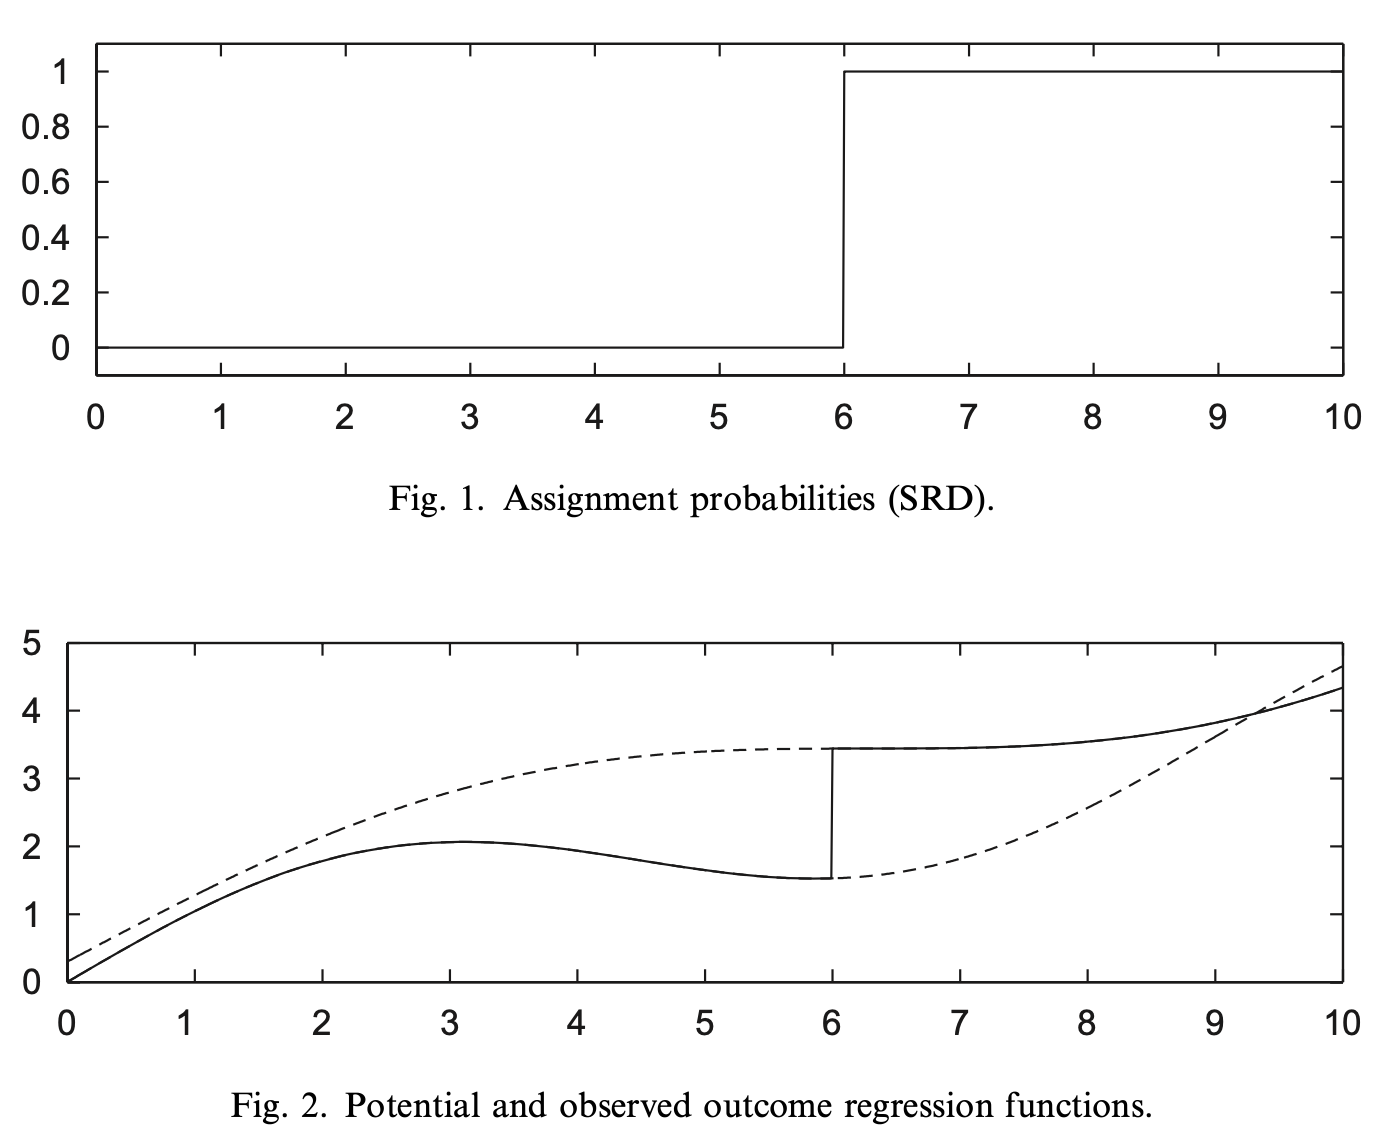
\includegraphics[scale=0.6]{fig1_2.png}
%	\caption{} %最终文档中希望显示的图片标题
%\label{fig1_2}
\end{figure}
Figs. 1 and 2  illustrate the identification strategy in the SRD setup. Based on artificial population values, we present in Fig. 1 the conditional probability of receiving the treatment, $\operatorname{Pr}(W=1 \mid X=x)$ against the covariate $x$. At $x=6$ the probability jumps from 0 to 1 . In Fig. 2, three conditional expectations are plotted. The two continuous lines (partly dashed, partly solid) in the figure are the conditional expectations of the two potential outcomes given the covariate, $\mu_{w}(x)=\mathbb{E}[Y(d) \mid X=x]$, for $w=0,1$. These two conditional expectations are continuous functions of the covariate. Note that we can only estimate $\mu_{0}(x)$ for $x<c$ and $\mu_{1}(x)$ for $x \geqslant c .$ In addition we plot the conditional expectation of the observed outcome
$$
\begin{aligned}
\mathbb{E}[Y \mid X=x]=& \mathbb{E}[Y \mid W=0, X=x] \cdot \operatorname{Pr}(W=0 \mid X=x) \\
&+\mathbb{E}[Y \mid W=1, X=x] \cdot \operatorname{Pr}(W=1 \mid X=x)
\end{aligned}
$$
in Fig. 2, indicated by a solid line. Although the two conditional expectations of the potential outcomes $\mu_{w}(x)$ are continuous, the conditional expectation of the observed outcome jumps at $x=c=6$.

\begin{remark}
	Now let us discuss the interpretation of $\lim _{x \downarrow c} \mathbb{E}\left[Y_{i} \mid X_{i}=x\right]-\lim _{x \uparrow c} \mathbb{E}\left[Y_{i} \mid X_{i}=x\right]$ as an average causal effect
	in more detail. In the SRD design, the widely used unconfoundedness assumption (e.g., Rosenbaum and Rubin, $1983 ;$ Imbens, 2004 ) underlying most matching-type estimators still holds:
	$$
	Y_{i}(0), Y_{i}(1) \perp \!\!\! \perp D_{i} \mid X_{i}
	$$
	This assumption holds in a trivial manner, because conditional on the covariates there is no variation in the treatment. However, this assumption cannot be exploited directly. The problem is that the second assumption that is typically used for matching-type approaches, the overlap assumption which requires that for all values of the covariates there are both treated and control units, or
	$$
	0<\operatorname{Pr}\left(D_{i}=1 \mid X_{i}=x\right)<1
	$$
	is fundamentally violated. In fact, for all values of $x$ the probability of assignment is either 0 or 1 , rather than always between 0 and 1 as required by the overlap assumption. As a result, there are no values of $x$ with Overlap.
\end{remark}

This implies there is an unavoidable need for extrapolation. However, in large samples the amount of extrapolation required to make inferences is arbitrarily small, as we only need to infer the conditional expectation of $Y(d)$ given the covariates $\varepsilon$ away from where it can be estimated. To avoid non-trivial extrapolation we focus on the average treatment effect at $X=c$ :
$$
\tau_{\mathrm{SRD}}=\mathbb{E}[Y(1)-Y(0) \mid X=c]=\mathbb{E}[Y(1) \mid X=c]-\mathbb{E}[Y(0) \mid X=c]
$$
By design, there are no units with $X_{i}=c$ for whom we observe $Y_{i}(0)$. We therefore will exploit the fact that we observe units with covariate values arbitrarily close to $c .^{2}$ In order to justify this averaging we make a smoothness assumption. Typically this assumption is formulated in terms of conditional expectations. Both following assumptions are stronger than required, as we will only use continuity at $x=c$: 
\begin{assu}[Continuity of Conditional Regression Functions] 
	~\\
	$\mathbb{E}[Y(0) \mid X=x]$ and $\mathbb{E}[Y(1) \mid X=x]$,
	are continuous in $x$.
\end{assu}

\begin{assu}[Continuity of Conditional Distribution Functions] 
	~\\
	More generally, one might want to assume that the conditional distribution function is smooth in the covariate. Let $F_{Y(d) \mid X}(y \mid x)=\operatorname{Pr}(Y(d) \leqslant y \mid X=x)$ denote the conditional distribution function of $Y(d)$ given $X$. Then the general version of the assumption is:
$F_{Y(0) \mid X}(y \mid x)$ and $F_{Y(1) \mid X}(y \mid x)$
are continuous in $x$ for all $y$.
\end{assu}
Under either assumption,
$$
\mathbb{E}[Y(0) \mid X=c]=\lim _{x \uparrow c} \mathbb{E}[Y(0) \mid X=x]=\lim _{x \uparrow c} \mathbb{E}[Y(0) \mid W=0, X=x]=\lim _{x \uparrow c} \mathbb{E}[Y \mid X=x]
$$
and similarly,
$$
\mathbb{E}[Y(1) \mid X=c]=\lim _{x \downarrow c} \mathbb{E}[Y \mid X=x]
$$
Thus, the average treatment effect at $c, \tau_{\mathrm{SRD}}$, satisfies
$$
\tau_{\mathrm{SRD}}=\lim _{x \downarrow c} \mathbb{E}[Y \mid X=x]-\lim _{x \uparrow c} \mathbb{E}[Y \mid X=x]
$$
The estimand is the difference of two regression functions at a point. Hence, if we try to estimate this object without parametric assumptions on the two regression functions, we do not obtain root- $N$ consistent estimators. Instead we get consistent estimators that converge to their limits at slower, nonparametric rates.
Identification argument is non-parametric: we don't need to assume anything about the distribution of $Y_{ i}(d)$ other than continuity of CEFs.


\subsection{Fuzzy RD}

\section{Practice}
\subsection{Sharp RD}
\subsubsection{Graphical Analyses and Specification Testing}
Graphical analyses should be an integral part of any RD analysis. The nature of RD designs suggests that the effect of the treatment of interest can be measured by the value of the discontinuity in the expected value of the outcome at a particular point. Inspecting the estimated version of this conditional expectation is a simple yet powerful way to visualize the identification strategy. Moreover, to assess the credibility of the RD strategy, it is useful to inspect two additional graphs for covariates and the density of the forcing variable. The estimators we discuss later use more sophisticated methods for smoothing but these basic plots will convey much of the intuition. 

\textbf{Outcomes by forcing variable:} 
The first plot is a histogram-type estimate of the average value of the outcome for different values of the forcing variable, the estimated counterpart to the solid line in Figs. 2 and 4 . For some binwidth $h$, and for some number of bins $K_{0}$ and $K_{1}$ to the left and right of the cutoff value, respectively, construct bins $\left(b_{k}, b_{k+1}\right]$, for $k=1, \ldots, K=K_{0}+K_{1}$, where
$$
b_{k}=c-\left(K_{0}-k+1\right) \cdot h
$$
Then calculate the number of observations in each bin
$$
N_{k}=\sum_{i=1}^{N} 1\left\{b_{k}<X_{i} \leqslant b_{k+1}\right\}
$$
and the average outcome in the bin
$$
\bar{Y}_{k}=\frac{1}{N_{k}} \cdot \sum_{i=1}^{N} Y_{i} \cdot 1\left\{b_{k}<X_{i} \leqslant b_{k+1}\right\}
$$
The first plot of interest is that of the $\bar{Y}_{k}$, for $k=1, \ldots, K$ against the mid point of the bins, $\tilde{b}_{k}=\left(b_{k}+b_{k+1}\right) / 2$. The question is whether around the threshold $c$ there is any evidence of a jump in the conditional mean of the outcome. The formal statistical analyses discussed below are essentially just sophisticated versions of this, and if the basic plot does not show any evidence of a discontinuity, there is relatively little chance that the more sophisticated analyses will lead to robust and credible estimates with statistically and substantially significant magnitudes. In addition to inspecting whether there is a jump at this value of the covariate, one should inspect the graph to see whether there are any other jumps in the conditional expectation of $Y$ given $X$ that are comparable to, or larger than, the discontinuity at the cutoff value. If so, and if one cannot explain such jumps on substantive grounds, it would call into question the interpretation of the jump at the threshold as the causal effect of the treatment. In order to optimize the visual clarity it is important to calculate averages that are not smoothed over the cutoff point.

\textbf{Covariates by forcing variable}
The second set of plots compares average values of other covariates in the $K$ bins. Specifically, let $Z_{i}$ be the $M$ -vector of additional covariates, with $m$ th element $Z_{i m} .$ Then calculate
$$
\bar{Z}_{k m}=\frac{1}{N_{k}} \cdot \sum_{i=1}^{N} Z_{i m} \cdot 1\left\{b_{k}<X_{i} \leqslant b_{k+1}\right\}
$$
The second plot of interest is that of the $\bar{Z}_{k m}$, for $k=1, \ldots, K$ against the mid point of the bins, $\tilde{b}_{k}$, for all $m=1, \ldots, M$. In the case of FRD designs, it is also particularly useful to plot the mean values of the treatment variable $D_{i}$ to make sure there is indeed a jump in the probability of treatment at the cutoff point (as in Fig. 3 . Plotting other covariates is also useful for detecting possible specification problems  in the case of either SRD or FRD designs.

One category of tests involves testing the null hypothesis of a zero average effect on pseudo outcomes known not to be affected by the treatment. Such variables includes covariates that are, by definition, not affected by the treatment. Such tests are familiar from settings with identification based on unconfoundedness assumptions (e.g., Heckman and Hotz, 1989; Rosenbaum, 1987; Imbens, 2004). In the RD setting, they have been applied by Lee et al. (2004) and others. In most cases, the reason for the discontinuity in the probability of the treatment does not suggest a discontinuity in the average value of covariates. If we find such a discontinuity, it typically casts doubt on the assumptions underlying the RD design. In principle, it may be possible to make the assumptions underlying the RD design conditional on covariates, and so a discontinuity in the conditional expectation of the covariates does not necessarily invalidate the approach. In practice, however, it is difficult to rationalize such discontinuities with the rationale underlying the RD approach.


\textbf{The Density of the forcing variable}
In the third graph, one should plot the number of observations in each bin, $N_{k}$, against the mid points $\tilde{b}_{k}$. This plot can be used to inspect whether there is a discontinuity in the distribution of the forcing variable $X$ at the threshold. Such discontinuity would raise the question of whether the value of this covariate was manipulated by the individual agent, invalidating the design. For example, suppose that the forcing variable is a test score. If individuals know the threshold and have the option of retaking the test, individuals with test scores just below the threshold may do so, and invalidate the design. Such a situation would lead to a discontinuity of the conditional density of the test score at the threshold, and thus be detectable in the kind of plots described here. 

The second test is conceptually somewhat different, and unique to the RD setting. McCrary (2007) suggests testing the null hypothesis of continuity of the density of the covariate that underlies the assignment at the discontinuity point, against the alternative of a jump in the density function at that point. Again, in principle, one does not need continuity of the density of X at c, but a discontinuity is suggestive of violations of the no-manipulation assumption. If in fact individuals partly manage to manipulate the value of X in order to be on one side of the cutoff rather than the other, one might expect to see a discontinuity in this density at the cutoff point. For example, if the variable underlying the assignment is age with a publicly known cutoff value c, and if age is self-reported, one might see relatively few individuals with a reported age just below c, and relatively many individuals with a reported age of just over c. Even if such discontinuities are not conclusive evidence of violations of the RD assumptions, at the very least, inspecting this density would be useful to assess whether it exhibits unusual features that may shed light on the plausibility of the design.


\subsubsection{Estimation}
% Nonparametric regression at the boundary
A simple model formalizes the RD idea. Potential outcomes can be described by a linear, constant-effects model
$$
\begin{aligned}
E\left[\mathrm{Y}_{0 i} \mid x_{i}\right] &=\alpha+\beta x_{i} \\
\mathrm{Y}_{1 i} &=\mathrm{Y}_{0 i}+\tau
\end{aligned}
$$
This leads to the regression,
$$
\mathrm{Y}_{i}=\alpha+\beta x_{i}+\tau \mathrm{D}_{i}+\eta_{i}
$$
where $\tau$ is the causal effect of interest. The key difference between this regression and others we've used
to estimate treatment effects  is that $\mathrm{D}_{i}$, the regressor of interest, is not only correlated
with $x_{i}$, it is a deterministic function of $x_{i}$. RD captures causal effects by distinguishing the nonlinear and
discontinuous function, $1\left(x_{i} \geq x_{0}\right)$, from the smooth and (in this case) linear function, $x_{i}$.

But what if the trend relation, $E\left[\mathrm{Y}_{0 i} \mid x_{i}\right]$, is nonlinear? To be precise, suppose that $E\left[\mathrm{Y}_{0 i} \mid x_{i}\right]=f\left(x_{i}\right)$ for
some reasonably smooth function, $f\left(x_{i}\right) .$  Now we can construct RD estimates by fitting
$$
\mathrm{Y}_{i}=f\left(x_{i}\right)+\tau \mathrm{D}_{i}+\eta_{i}
$$
where again, $\mathrm{D}_{i}=1\left(x_{i} \geq x_{0}\right)$ is discontinuous in $x_{i}$ at $x_{0} .$ As long as $f\left(x_{i}\right)$ is continuous in a neighborhood
of $x_{0}$, it should be possible to estimate a model like $\sqrt{6.1 .3}$, even with a flexible functional form for $f\left(x_{i}\right)$. For
example, modeling $f\left(x_{i}\right)$ with a $p^{t h}$ -order polynomial, RD estimates can be constructed from the regression
\begin{equation}\label{s}
\mathrm{Y}_{i}=\alpha+\beta_{1} x_{i}+\beta_{2} x_{i}^{2}+\ldots+\beta_{p} x_{i}^{p}+\tau \mathrm{D}_{i}+\eta_{i}
\end{equation}

A generalization of RD  allows different trend functions for $E\left[\mathrm{Y}_{0 i} \mid x_{i}\right]$ and $E\left[\mathrm{Y}_{1 i} \mid x_{i}\right] .$
Modeling both of these CEFs with $p^{\text {th }}$ -order polynomials, we have
$$
\begin{aligned}
&E\left[\mathrm{Y}_{0 i} \mid x_{i}\right]=f_{0}\left(x_{i}\right)=\alpha+\beta_{01} \tilde{x}_{i}+\beta_{02} \tilde{x}_{i}^{2}+\ldots+\beta_{0 p} \tilde{x}_{i}^{p} \\
&E\left[\mathrm{Y}_{1 i} \mid x_{i}\right]=f_{1}\left(x_{i}\right)=\alpha+\tau+\beta_{11} \tilde{x}_{i}+\beta_{12} \tilde{x}_{i}^{2}+\ldots+\beta_{1 p} \tilde{x}_{i}^{p}
\end{aligned}
$$
where $\tilde{x}_{i} \equiv x_{i}-x_{0} . \quad$ Centering $x_{i}$ at $x_{0}$ is just a normalization; it ensures that the treatment effect at
$x_{i}=x_{0}$ is still the coefficient on $\mathrm{D}_{i}$ in the regression model with interactions (because you do not have to add values of the $D_{i}$ interacted with $X$ to get the treatment effect at $x_{0}$).

To derive a regression model that can be used to estimate the effects interest in this case, we use the fact
that $\mathrm{D}_{i}$ is a deterministic function of $x_{i}$ to write
$$
E\left[\mathrm{Y}_{i} \mid x_{i}\right]=E\left[\mathrm{Y}_{0 i} \mid x_{i}\right]+E\left[\mathrm{Y}_{1 i}-\mathrm{Y}_{0 i} \mid x_{i}\right] \mathrm{D}_{i}
$$
Substituting polynomials for conditional expectations, we then have
\begin{equation}\label{g}
\begin{aligned}
\mathrm{Y}_{i}=& \alpha+\beta_{01} \tilde{x}_{i}+\beta_{02} \tilde{x}_{i}^{2}+\ldots+\beta_{0 p} \tilde{x}_{i}^{p} \\
&+\tau \mathrm{D}_{i}+\beta_{1}^{*} \mathrm{D}_{i} \tilde{x}_{i}+\beta_{2}^{*} \mathrm{D}_{i} \tilde{x}_{i}^{2}+\ldots+\beta_{p}^{*} \mathrm{D}_{i} \tilde{x}_{i}^{p}+\eta_{i}
\end{aligned}
\end{equation}
where $\beta_{1}^{*}=\beta_{11}-\beta_{01}, \beta_{2}^{*}=\beta_{12}-\beta_{02}$, and $\beta_{p}^{*}=\beta_{1 p}-\beta_{0 p}$ and the error term, $\eta_{i}$, is the CEF residual. 

Equation \ref{s} is a special case of \ref{g} where $\beta_{1}^{*}=\beta_{2}^{*}=\beta_{p}^{*}=0 .$ In the more general model, the treatment effect at $x_{i}-x_{0}=c>0$ is $\tau+\beta_{1}^{*} c+\beta_{2}^{*} c^{2}+\ldots+\beta_{p}^{*} c^{p}$, while the treatment effect at $x_{0}$ is $\tau$
The model with interactions has the attraction that it imposes no restrictions on the underlying conditional
mean functions. But in our experience, RD estimates of $\tau$ based on the simpler model, $6.1 .4)$, usually turn
out to be similar to those based on \ref{g}.

The validity of RD estimates based on \ref{s} or \ref{g} turns on whether polynomial models provide an
adequate description of $E\left[\mathrm{Y}_{0 i} \mid \mathrm{X}_{i}\right] .$ If not, then what looks like a jump due to treatment might simply be an
unaccounted-for nonlinearity in the counterfactual conditional mean function.
\begin{figure}[H]
	\centering
	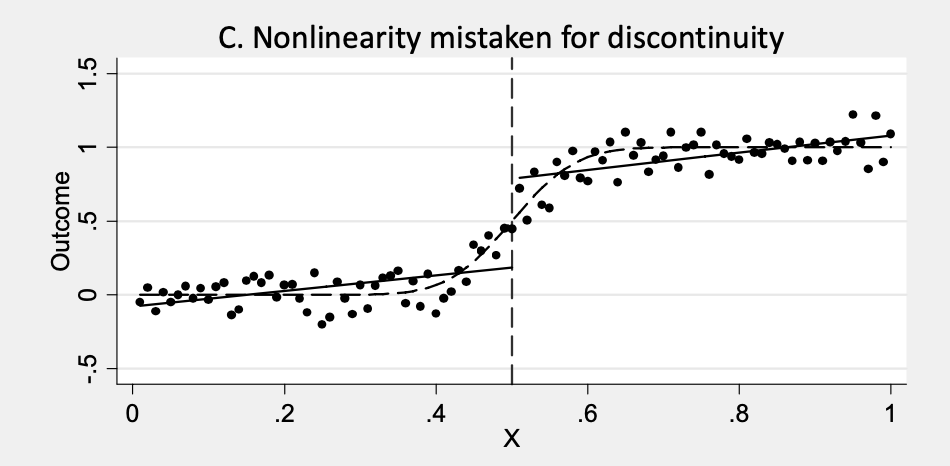
\includegraphics[scale=0.6]{mis.png}
	%	\caption{} %最终文档中希望显示的图片标题
	%\label{fig1_2}
\end{figure}
 This possibility is that a sharp turn in $E\left[\mathrm{Y}_{0 i} \mid x_{i}\right]$ might be mistaken for a jump from
one regression line to another. To reduce the likelihood of such mistakes, we can look only at data in a
neighborhood around the discontinuity, say the interval $\left[x_{0}-\delta, x_{0}+\delta\right]$ for some small number $\delta$. Then we
have
$$
\begin{aligned}
&E\left[\mathrm{Y}_{i} \mid x_{0}-\delta<x_{i}<x_{0}\right] \simeq E\left[\mathrm{Y}_{0 i} \mid x_{i}=x_{0}\right] \\
&E\left[\mathrm{Y}_{i} \mid x_{0}<x_{i}<x_{0}+\delta\right] \simeq E\left[\mathrm{Y}_{1 i} \mid x_{i}=x_{0}\right]
\end{aligned}
$$
so that
\begin{equation}\label{ate}
\lim _{\delta \rightarrow 0} E\left[\mathrm{Y}_{i} \mid x_{0}<x_{i}<x_{0}+\delta\right]-E\left[\mathrm{Y}_{i} \mid x_{0}-\delta<x_{i}<x_{0}\right]=E\left[\mathrm{Y}_{1 i}-\mathrm{Y}_{0 i} \mid x_{i}=x_{0}\right]
\end{equation}
In other words, comparisons of average outcomes in a small enough neighborhood to the left and right of $x_{0}$
should provide an estimate of the treatment effect that does not depend on the correct specification of a model
for $E\left[\mathrm{Y}_{0 i} \mid x_{i}\right]$. Moreover, the validity of this nonparametric estimation strategy does not turn on the constant
effects assumption, $\mathrm{y}_{1 i}-\mathrm{Y}_{0 i}=\tau$; the estimand in \ref{ate} is the average causal effect, $E\left[\mathrm{Y}_{1 i}-\mathrm{Y}_{0 i} \mid x_{i}=x_{0}\right]$.

\subsubsection{Covariates}
Often there are additional covariates available in addition to the forcing covariate that is the basis of the assignment mechanism. These covariates can be used to eliminate small sample biases present in the basic specification, and improve the precision. In addition, they can be useful for evaluating the plausibility of the identification strategy.  Let the additional vector of covariates be denoted by $Z_{i}$. We make three observations on the role of these additional covariates. The first and most important point is that the presence of these covariates rarely changes the identification strategy. Typically, the conditional distribution of the covariates $Z$ given $X$ is continuous at $x=c .$ In fact, one may wish to test for discontinuities at that value of $x$ in order to assess the plausibility of the identification strategy. If such discontinuities in other covariates are found, the justification of the identification strategy may be questionable. If the conditional distribution of $Z$ given $X$ is continuous at $x=c$, then including $Z$ in the regression will have little effect on the expected value of the estimator for $\tau$, since conditional on $X$ being close to $c$, the additional covariates $Z$ are independent of $W$.

The second point is that even though the presence of $Z$ in the regression does not affect any bias when $X$ is very close to $c$, in practice we often include observations with values of $X$ not too close to $c$. In that case, including additional covariates may eliminate some bias that is the result of the inclusion of these additional observations.

Third, the presence of the covariates can improve precision if $Z$ is correlated with the potential outcomes. This is the standard argument, which also supports the inclusion of covariates in analyses of randomized experiments. In practice the variance reduction will be relatively small unless the contribution to the $R^{2}$ from the additional regressors is substantial.

\subsubsection{Bandwidth choice}
An important issue in practice is the selection of the smoothing parameter, the binwidth $h$. In general there are two approaches to choose bandwidths. A first approach consists of characterizing the optimal bandwidth in terms of the unknown joint distribution of all variables. The relevant components of this distribution can then be estimated, and plugged into the optimal bandwidth function. The second approach, on which we focus here, is based on a cross-validation procedure. The specific methods discussed here are similar to those developed by Ludwig and Miller (2005, 2007). In particular, their proposals, like ours, are aimed specifically at estimating the regression function at the boundary. Initially we focus on the SRD case, and in Section $5.2$ we extend the recommendations to the FRD setting.

To set up the bandwidth choice problem we generalize the notation slightly. In the SRD setting we are interested in
$$
\tau_{\mathrm{SRD}}=\lim _{x \downarrow c} \mu(x)-\lim _{x \uparrow c} \mu(x) .
$$
We estimate the two terms as
$$
\lim _{x \downarrow c} \widehat{\mu}(x)=\hat{\alpha}_{r}(c)
$$
and
$$
\lim _{x \uparrow c} \widehat{\mu}(x)=\hat{\alpha}_{1}(c)
$$
where $\hat{\alpha}_{1}(x)$ and $\hat{\beta}_{1}(x)$ solve
$$
\left(\hat{\alpha}_{1}(x), \hat{\beta}_{1}(x)\right)=\arg \min _{\alpha, \beta} \sum_{j \mid x-h<X_{j}<x}\left(Y_{j}-\alpha-\beta \cdot\left(X_{j}-x\right)\right)^{2}
$$
and $\hat{\alpha}_{\mathrm{r}}(x)$ and $\hat{\beta}_{\mathrm{r}}(x)$ solve
$$
\left(\hat{\alpha}_{\mathrm{r}}(x), \hat{\beta}_{\mathrm{r}}(x)\right)=\arg \min _{\alpha, \beta} \sum_{j \mid x<X_{j}<x+h}\left(Y_{j}-\alpha-\beta \cdot\left(X_{j}-x\right)\right)^{2}
$$
Let us focus first on estimating $\lim _{x \downarrow c} \mu(x) .$ For estimation of this limit we are interested in the bandwidth $h$ that minimizes
\begin{equation}\label{Q1}
Q_{\mathrm{r}}(x, h)=\mathbb{E}\left[\left(\lim _{z \downarrow x} \mu(z)-\hat{\alpha}_{\mathrm{r}}(x)\right)^{2}\right]
\end{equation}
at $x=c .$ In principle this could be different from the bandwidth that minimizes the corresponding criterion on the left-hand side,
\begin{equation}\label{Q2}
Q_{1}(x, h)=\mathbb{E}\left[\left(\lim _{z \uparrow x} \mu(z)-\hat{\alpha}_{1}(x)\right)^{2}\right]
\end{equation}
at $x=c .$ However, we will focus on a single bandwidth for both sides of the threshold, and therefore focus on minimizing
$$
\begin{aligned}
Q(c, h) &=\frac{1}{2} \cdot\left(Q_{1}(c, h)+Q_{\mathrm{r}}(c, h)\right) \\
&=\frac{1}{2} \cdot\left(\mathbb{E}\left[\left(\lim _{x \uparrow c} \mu(x)-\hat{\alpha}_{1}(c)\right)^{2}\right]+\mathbb{E}\left[\left(\lim _{x \downarrow c} \mu(x)-\hat{\alpha}_{\mathrm{r}}(c)\right)^{2}\right]\right)
\end{aligned}
$$

We now discuss two methods for choosing the bandwidth.

For a given binwidth $h$, let the estimated regression function at $x$ be
$$
\hat{\mu}(x)= \begin{cases}\hat{\alpha}_{1}(x) & \text { if } x<c \\ \hat{\alpha}_{\mathrm{r}}(x) & \text { if } x \geqslant c\end{cases}
$$
where $\hat{\alpha}_{1}(x), \hat{\beta}_{1}(x), \hat{\alpha}_{\mathrm{r}}(x)$, and $\hat{\beta}_{\mathrm{r}}(x)$ solve \ref{Q1} and \ref{Q2}. Note that in order to mimic the fact that we are interested in estimation at the boundary, we only use the observations on one side of $x$ in order to estimate the regression function at $x$, rather than the observations on both sides of $x$, that is, observations with $x-h<X_{j}<x+h .$ In addition, the strict inequality in the definition implies that $\hat{\mu}(x)$ evaluated at $x=X_{i}$ does not depend on $Y_{i}$. Now define the cross-validation criterion as
\begin{equation}\label{CVy}
\mathrm{CV}_{Y}(h)=\frac{1}{N} \sum_{i=1}^{N}\left(Y_{i}-\hat{\mu}\left(X_{i}\right)\right)^{2}
\end{equation}
with the corresponding cross-validation choice for the binwidth
$$
h_{\mathrm{CV}}^{\mathrm{opt}}=\arg \min _{h} \mathrm{CV}_{Y}(h)
$$
The expected value of this cross-validation function is, ignoring the term that does not involve $h$, equal to $\mathbb{E}\left[\mathrm{CV}_{Y}(h)\right]=C+\mathbb{E}[Q(X, h)]=C+\int Q(x, h) f_{X} \mathrm{~d} x .$ Although the modification to estimate the regression
using one-sided kernels mimics more closely the estimand of interest, this is still not quite what we are interested in. Ultimately, we are solely interested in estimating the regression function in the neighborhood of a single point, the threshold $c$, and thus in minimizing $Q(c, h)$, rather than $\int_{x} Q(x, h) f_{X}(x) \mathrm{d} x$. If there are quite a few observations in the tails of the distribution, minimizing the criterion in \ref{CVy} may lead to larger bins than is optimal for estimating the regression function around $x=c$, if $c$ is in the center of the distribution. We may therefore wish to minimize the cross-validation criterion after first discarding observations from the tails. Let $q_{X, \delta, 1}$ be the $\delta$ quantile of the empirical distribution of $X$ for the subsample with $X_{i}<c$, and let $q_{X, 1-\delta, \mathrm{r}}$ be the $1-\delta$ quantile of the empirical distribution of $X$ for the subsample with $X_{i} \geqslant c$. Then, we may wish to use the criterion
$$
\mathrm{CV}_{Y}^{\delta}(h)=\frac{1}{N} \sum_{i: q_{X, \delta, 1} \leqslant X_{i} \leqslant q_{X, 1-\delta, \mathrm{r}}}\left(Y_{i}-\hat{\mu}\left(X_{i}\right)\right)^{2}
$$
The modified cross-validation choice for the bandwidth is
$$
h_{\mathrm{CV}}^{\delta, \mathrm{opt}}=\arg \min _{h} \mathrm{CV}_{Y}^{\delta}(h) .
$$
The modified cross-validation function has expectation, again ignoring terms that do not involve $h$, proportional to $\mathbb{E}\left[Q(X, h) \mid q_{X, \delta, 1}<X<q_{X, 1-\delta, \mathrm{r}}\right]$. Choosing a smaller value of $\delta$ makes the expected value of the criterion closer to what we are ultimately interested in, that is, $Q(c, h)$, but has the disadvantage of leading to a noisier estimate of $\mathbb{E}\left[\mathrm{CV}_{Y}^{\delta}(h)\right]$. In practice, one may wish to choose $\delta=\frac{1}{2}$, and discard $50 \%$ of the observations on either side of the threshold, and afterwards assess the sensitivity of the bandwidth choice to the choice of $\delta$. Ludwig and Miller (2005) implement this by using only data within $5 \%$ points of the threshold on either side. Note that, in principle, we can use a different binwidth on either side of the cutoff value. However, it is likely that the density of the forcing variable $x$ is similar on both sides of the cutoff point. If, in addition, the curvature is similar on both sides close to the cutoff point, then in large samples the optimal binwidth will be similar on both sides. Hence, the benefits of having different binwidths on the two sides may not be sufficient to balance the disadvantage of the additional noise in estimating the optimal value from a smaller sample.


\subsubsection{Order of polynomial}
 The simplest way of implementing polynomial regressions and computing standard errors is to run a pooled regression. For example, in the case of a third order polynomial regression, we would have
 $$
 \begin{aligned}
 Y=& \alpha_{l}+\tau D+\beta_{l 1}(X-c) \\
 &+\beta_{l 2}(X-c)^{2}+\beta_{l 3}(X-c)^{3} \\
 &+\left(\beta_{r 1}-\beta_{l 1}\right) D(X-c) \\
 &+\left(\beta_{r 2}-\beta_{l 2}\right) D(X-c)^{2} \\
 &+\left(\beta_{r 3}-\beta_{l 3}\right) D(X-c)^{3}+\varepsilon
 \end{aligned}
 $$
 While it is important to report a number of specifications to illustrate the robustness of the results, it is often useful to have some more formal guidance on the choice of the order of the polynomial. Starting with van der Klaauw (2002), one approach has been to use a generalized cross-validation procedure suggested in the literature on nonparametric series estimators. ${ }^{36}$ One special case of generalized cross-validation (used by Dan
 A. Black, Jose Galdo, and Smith $(2007 a)$, for example), which we also use in our empirical example, is the well known Akaike information criterion (AIC) of model selection. In a regression context, the AIC is given by
 $$
 A I C=N \ln \left(\hat{\sigma}^{2}\right)+2 p
 $$
 where $\hat{\sigma}^{2}$ is the mean squared error of the regression, and $p$ is the number of parameters in the regression model (order of the polynomial plus one for the intercept).
 
 One drawback of this approach is that it does not provide a very good sense of how  a particular parametric model (say a cubic model) compares relative to a more general nonparametric alternative. In the context of the RD design, a natural nonparametric alternative is the set of unrestricted means of the outcome variable by bin used to graphically depict the data in section $4.1$. Since one virtue of polynomial regressions is that they provide a smoothed version of the graph, it is natural to ask how well the polynomial model fits the unrestricted graph. A simple way of implementing the test is to add the set of bin dummies to the polynomial regression and jointly test the significance of the bin dummies. For example, in a first order polynomial model (linear regression), the test can be computed by including $K-2$ bin dummies $B_{k}$, for $k=2$ to $K-1$, in the model
 $$
 \begin{aligned}
 Y=& \alpha_{l}+\tau D+\beta_{l 1}(X-c) \\
 &+\left(\beta_{r 1}-\beta_{l 1}\right) D(X-c) \\
 &+\sum_{k=2}^{K-1} \phi_{k} B_{k}+\varepsilon
 \end{aligned}
 $$
 and testing the null hypothesis that $\phi_{2}=\phi_{3}=\ldots=\phi_{K-1}=0$. Note that two of
 the dummies are excluded because of collinearity with the constant and the treatment dummy, $D .^{37}$ In terms of specification choice procedure, the idea is to add a higher order term to the polynomial until the bin dummies are no longer jointly significant.
 
 Another major advantage of this procedure is that testing whether the bin dummies are significant turns out to be a test for the presence of discontinuities in the regression function at points other than the cutoff point. In that sense, it provides a falsification test of the RD design by examining whether there are other unexpected discontinuities in the regression function at randomly chosen points (the bin thresholds). To see this, rewrite $\sum_{k=1}^{K} \phi_{k} B_{k}$ as
 $$
 \sum_{k=1}^{K} \phi_{k} B_{k}=\phi_{1}+\sum_{k=2}^{K}\left(\phi_{k}-\phi_{k-1}\right) B_{k}^{+}
 $$
 where $B_{k}^{+}=\sum_{j=k}^{K} B_{j}$ is a dummy variable indicating that the observation is in bin $k$ or above, i.e., that the assignment variable $X$ is above the bin cutoff $b_{k}$. Testing whether all the $\phi_{k}-\phi_{k-1}$ are equal to zero is equivalent to testing that all the $\phi_{k}$ are the same (the above test), which amounts to testing that the regression line does not jump at the bin thresholds $b_{k}$.
 
 Broadly speaking, the goodness-of-fit tests do a very good job ruling out clearly misspecified models, like the zero order poly- nomials with large bandwidths that yield upward biased estimates of the treatment effect.  One set of models the goodness-of- fit test does not rule out, however, is higher order polynomial models with small bandwidths that tend to be imprecisely estimated as they “overfit” the data. Looking informally at both the fit of the model (goodness-of-fit test) and the precision of the estimates (standard errors) suggests the following strategy: use higher order polynomials for large bandwidths, lower order polynomials for small bandwidths, since the latter specification passes the goodness-of-fit test for these very small bandwidths. Interestingly, this informal approach more or less corresponds to what is suggested by the AIC. In this specific example, it seems that given a specific bandwidth, the AIC provides reasonable suggestions on which order of the polynomial to use.
 
% \subsubsection{Specification testing}
 
\subsection{Fuzzy RD}


\subsection{Recommended Checklist}


\section{Example}
\subsection{Sharp RD}

\subsection{Fuzzy RD}






\newpage 
%\bibliographystyle{plain}
\bibliography{bibtex}
\end{document}

